\newpage
\section{System Design}
\subsection{Design Approach}
We have used both Function oriented and Object oriented Approach in our project. As with function oriented we can have easy flow of information and in object oriented we can use concepts like information hiding, benefits of constructor and destructor etc.
\begin{figure}[H]
    \centering
    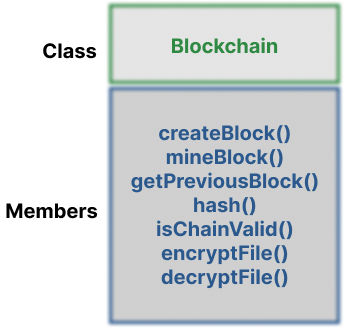
\includegraphics[scale=0.55]{images/oops.png}\\[0.5cm]
    \caption{Design Approach}
    \label{fig:my_label}
\end{figure}

Design approach includes object oriented design as well as function oriented design where we have created \textbf{blockchain} class where data members are: 
\begin{itemize}
    \item Create Block
    \item Mine Block
    \item Get Previous Block
    \item Hash
    \item Is chain Valid
    \item Encrypt File
    \item Decrypt file
\end{itemize}

\textbf{Functions included are}:
\begin{itemize}
    \item login(): Login function which is used to redirect to the user to login page.
    \item logout(): Student or Admin can logout using this function
    \item AddUser(): Admin can add user by using this function through the interface.
    \item Dashboard(): The main page is our Dashboard page which is used to see the certificates of particular user,
    \item getchain(): One can use to see the block chain that has been made till time.
    \item isvalid(): It will return True if the chain is valid else False.
    \item uploadfile(): It is used to upload the file to IPFS.
    \item authoritycheck(): It is used to check the authority whether a user is admin or student.
\end{itemize}

% \subsection{Detail Design}
\subsection{System Design} 
\begin{figure}[H]
    \centering
    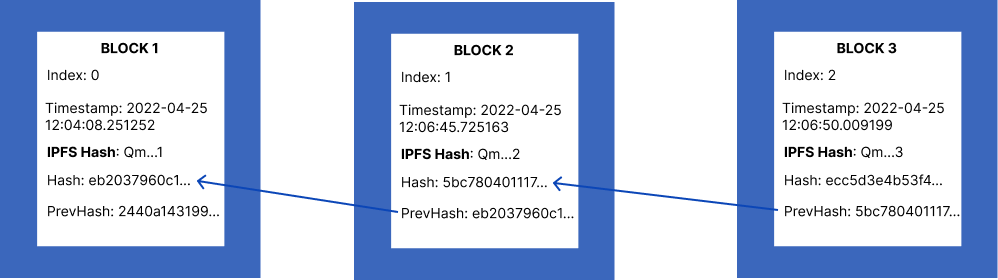
\includegraphics[scale=0.4]{images/ipfs_blockchain.png}\\[0.5cm]
    \caption{Blockchain Design}
    \label{fig:my_label}
\end{figure}

Blockchain is how the data is structured. A blockchain collects information together in groups, known as blocks, that hold sets of information. Blocks have certain storage capacities and, when filled, are closed and linked to the previously filled block, forming a chain of data known as the blockchain. All new information that follows that freshly added block is compiled into a newly formed block that will then also be added to the chain once filled.

\begin{figure}[H]
    \centering
    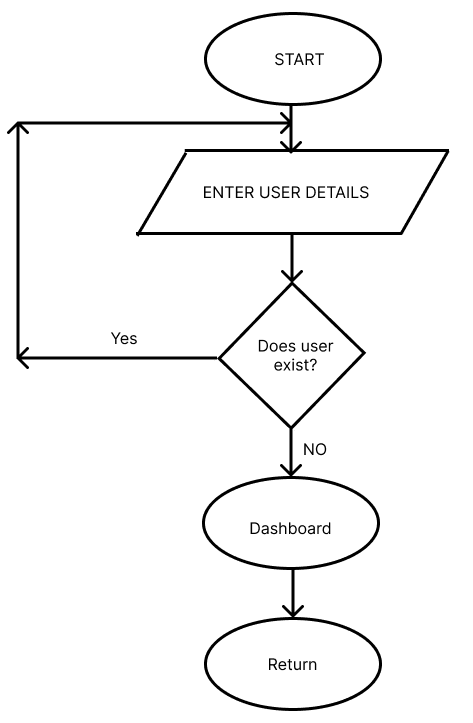
\includegraphics[scale=0.4]{images/user_flowchart.png}\\[0.5cm]
    \caption{Add User Page}
    \label{fig:my_label}
\end{figure}

\noindent
In add user page, admin adds user details of the student and if the student already exist then re-enter the correct student details and if it does not exist then student will be added.

\begin{figure}[H]
    \centering
    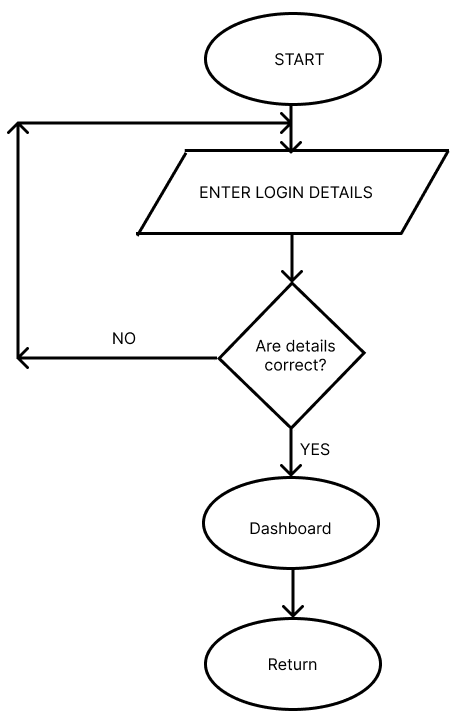
\includegraphics[scale=0.4]{images/login_flowchart.png}\\[0.5cm]
    \caption{Login Page}
    \label{fig:my_label}
\end{figure}

\noindent
In login page, student enters his/her login details and he/she is validated on the basis of username and password and is redirected to dashboard.

\begin{figure}[H]
    \centering
    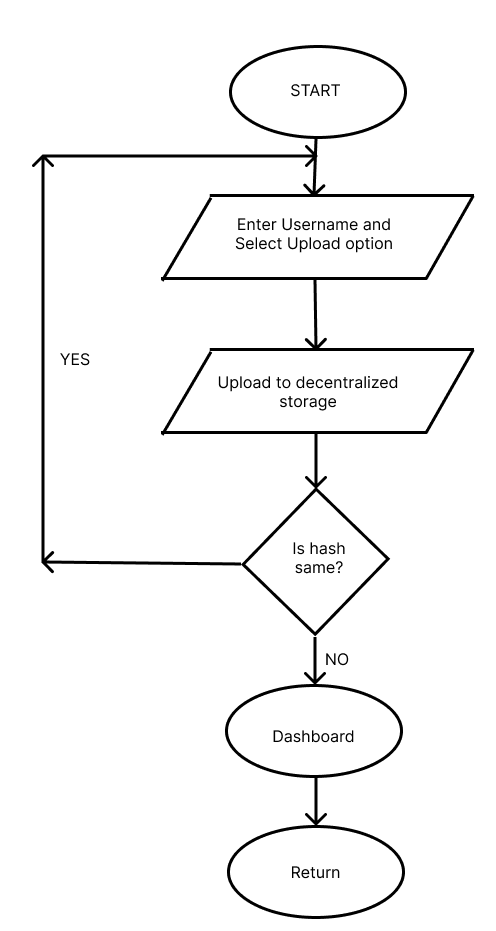
\includegraphics[scale=0.4]{images/upload_flowchart.png}\\[0.5cm]
    \caption{Upload Page}
    \label{fig:my_label}
\end{figure}

\noindent
In upload page, admin enters username of the student and uploads the transcripts in the IPFS. After this, user gets the access of the transcripts after getting file uploaded.

\begin{figure}[H]
    \centering
    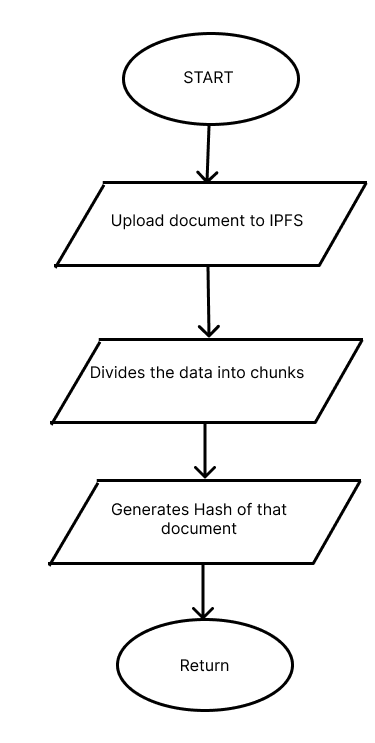
\includegraphics[scale=0.4]{images/IPFS_flowchart.png}\\[0.5cm]
    \caption{IPFS Design}
    \label{fig:my_label}
\end{figure}

\noindent
Here after uploading file from the user interface, the file is uploaded on the IPFs i.e. Interplanetary File System and since it is decentralized storage so all peers those have access to the file can access the transcripts from IPFS.

\subsection{User Interface Design} 

\begin{figure}[H]
    \centering
    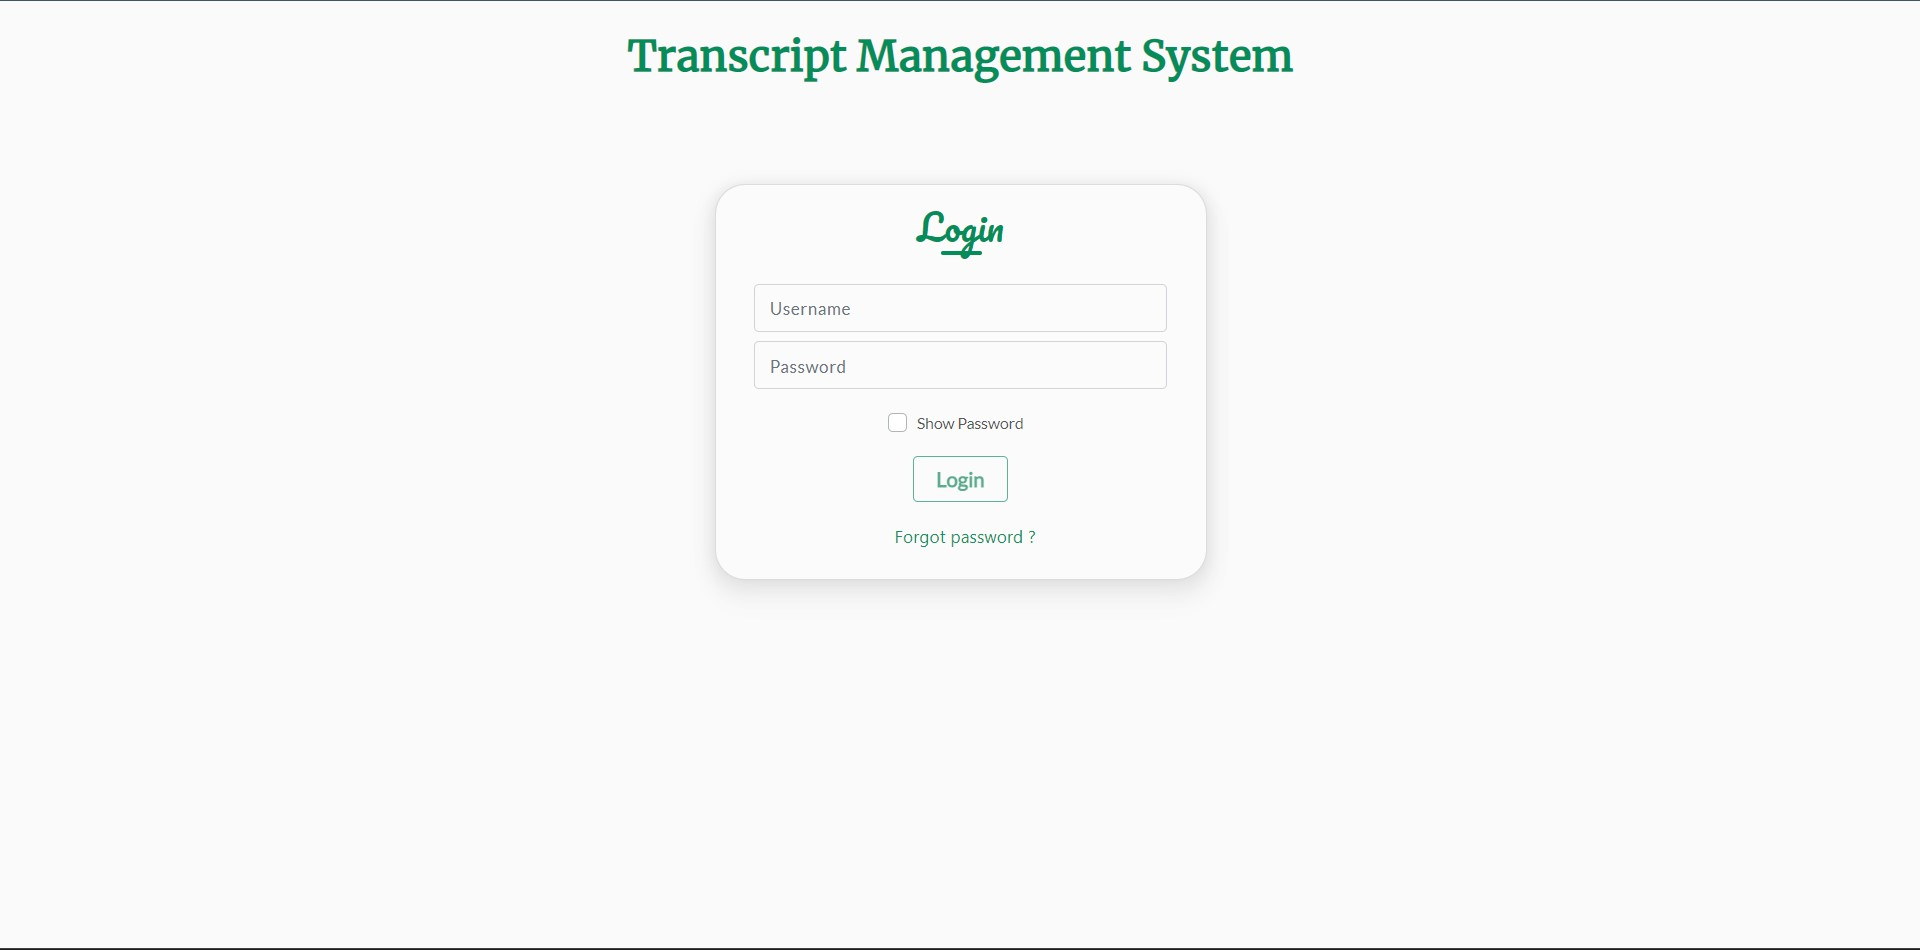
\includegraphics[scale=0.32]{images/login.jpg}\\[0.5cm]
    \caption{Login Design}
    \label{fig:my_label}
\end{figure}

\noindent
In login page, student enters his/her login details and he/she is validated on the basis of username and password and is redirected to dashboard.

\begin{figure}[H]
    \centering
    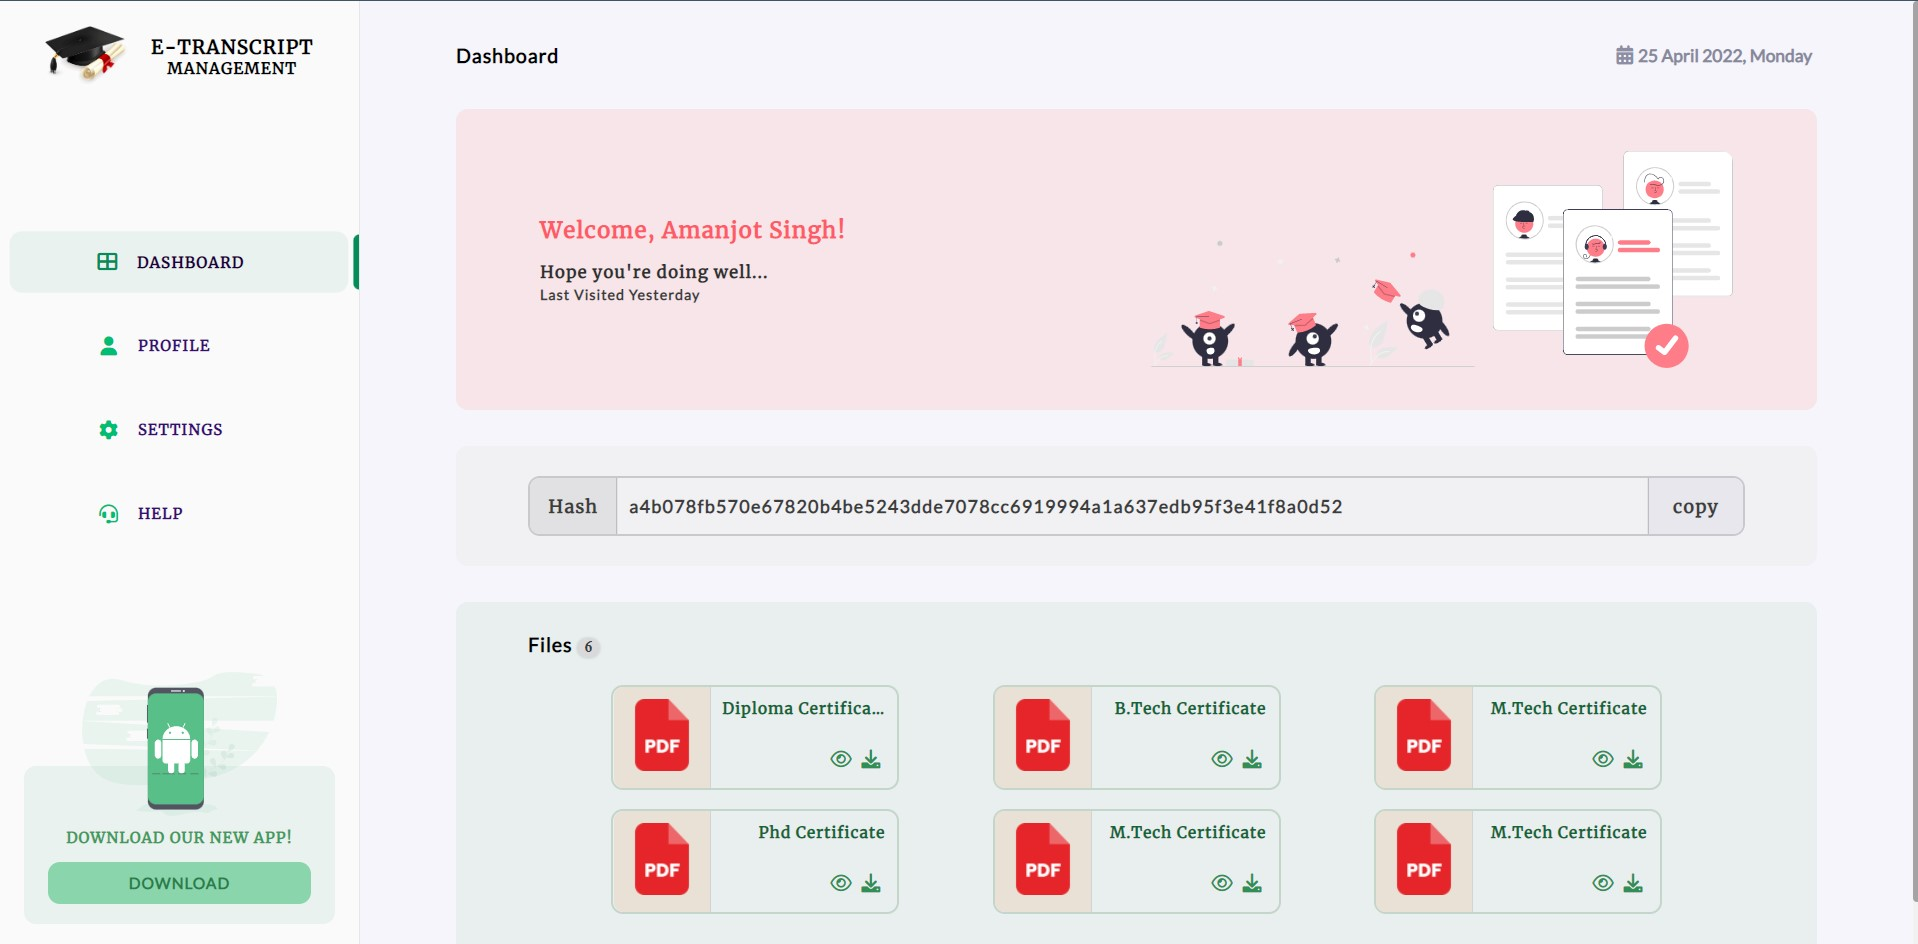
\includegraphics[scale=0.32]{images/Dashboard.jpg}\\[0.5cm]
    \caption{Dashboard Design}
    \label{fig:my_label}
\end{figure}

\noindent
In dashboard, students can access their transcripts and can share the access to anyone they want without any delay.
They can download and view direct from decentralized storage.

\begin{figure}[H]
    \centering
    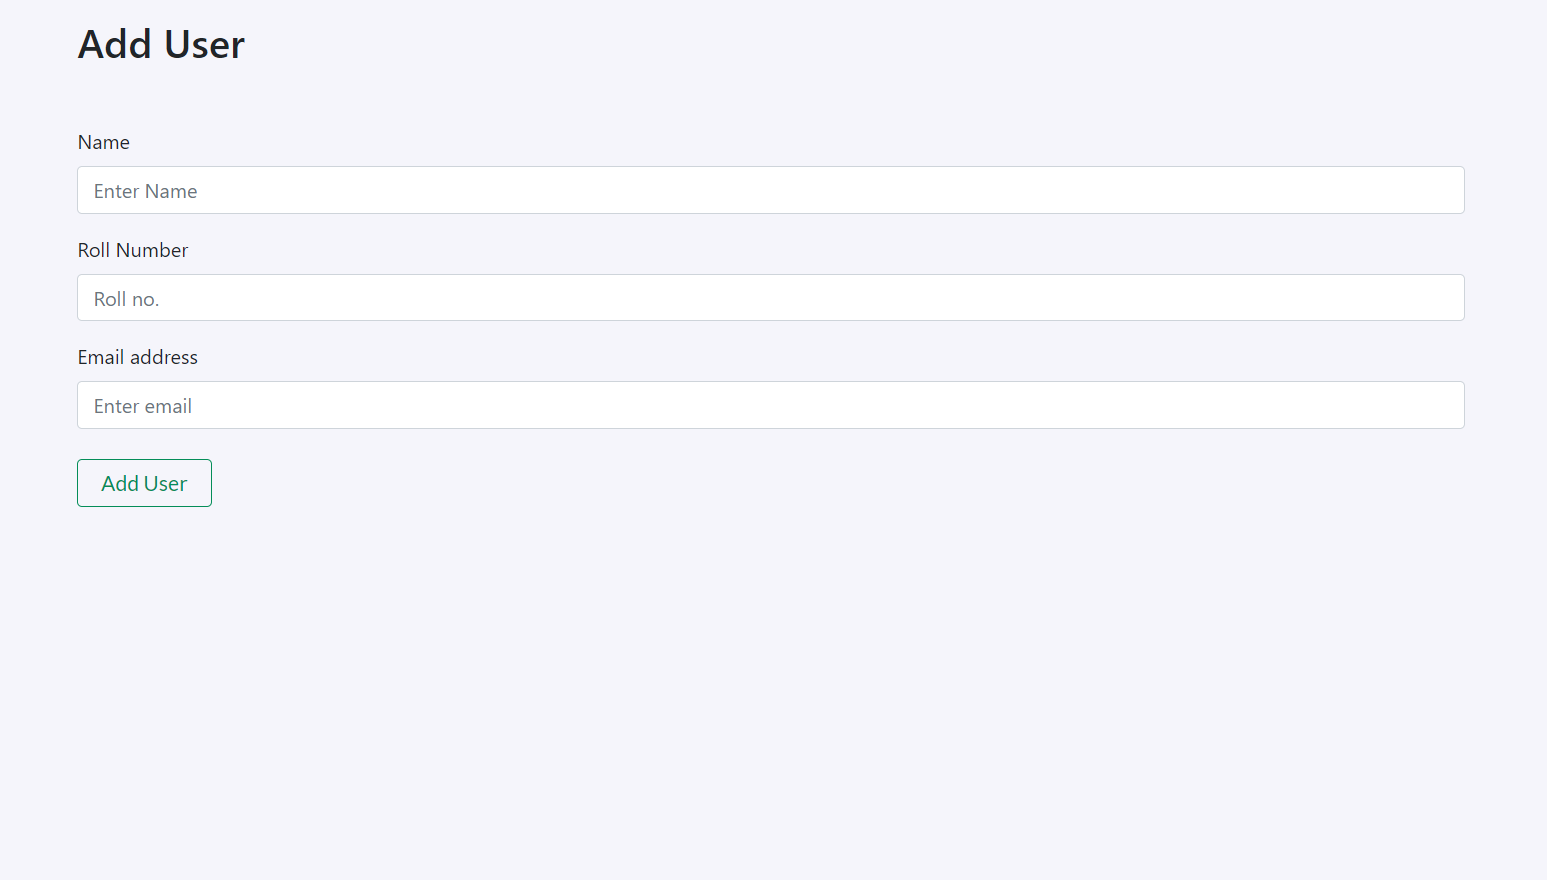
\includegraphics[scale=0.4]{images/add_user.png}\\[0.5cm]
    \caption{Add User Design}
    \label{fig:my_label}
\end{figure}

\noindent
In add user page, user can be added to access the uploaded transcripts of that particular user only.

\begin{figure}[H]
    \centering
    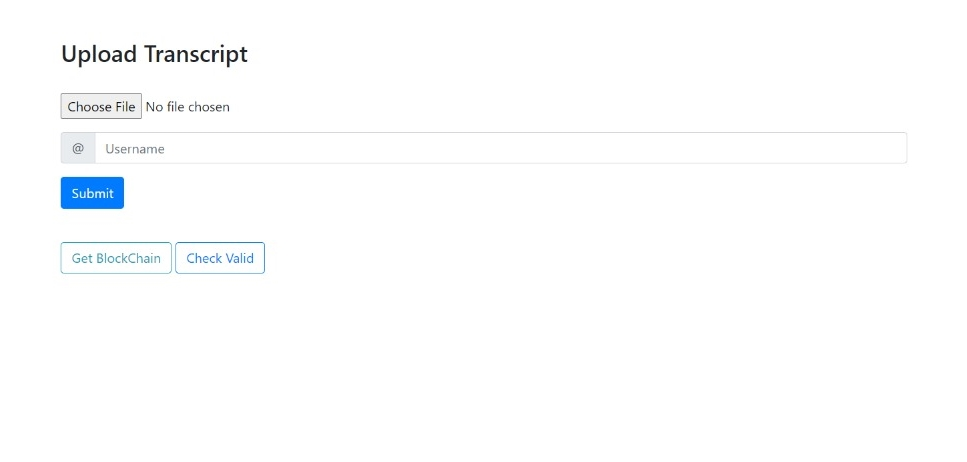
\includegraphics[scale=0.53]{images/upload_page.jpeg}\\[0.5cm]
    \caption{Upload Page Design}
    \label{fig:my_label}
\end{figure}

\noindent
Upload page is designed for admins to upload the transcripts and show them to that particular user only.

\begin{figure}[H]
    \centering
    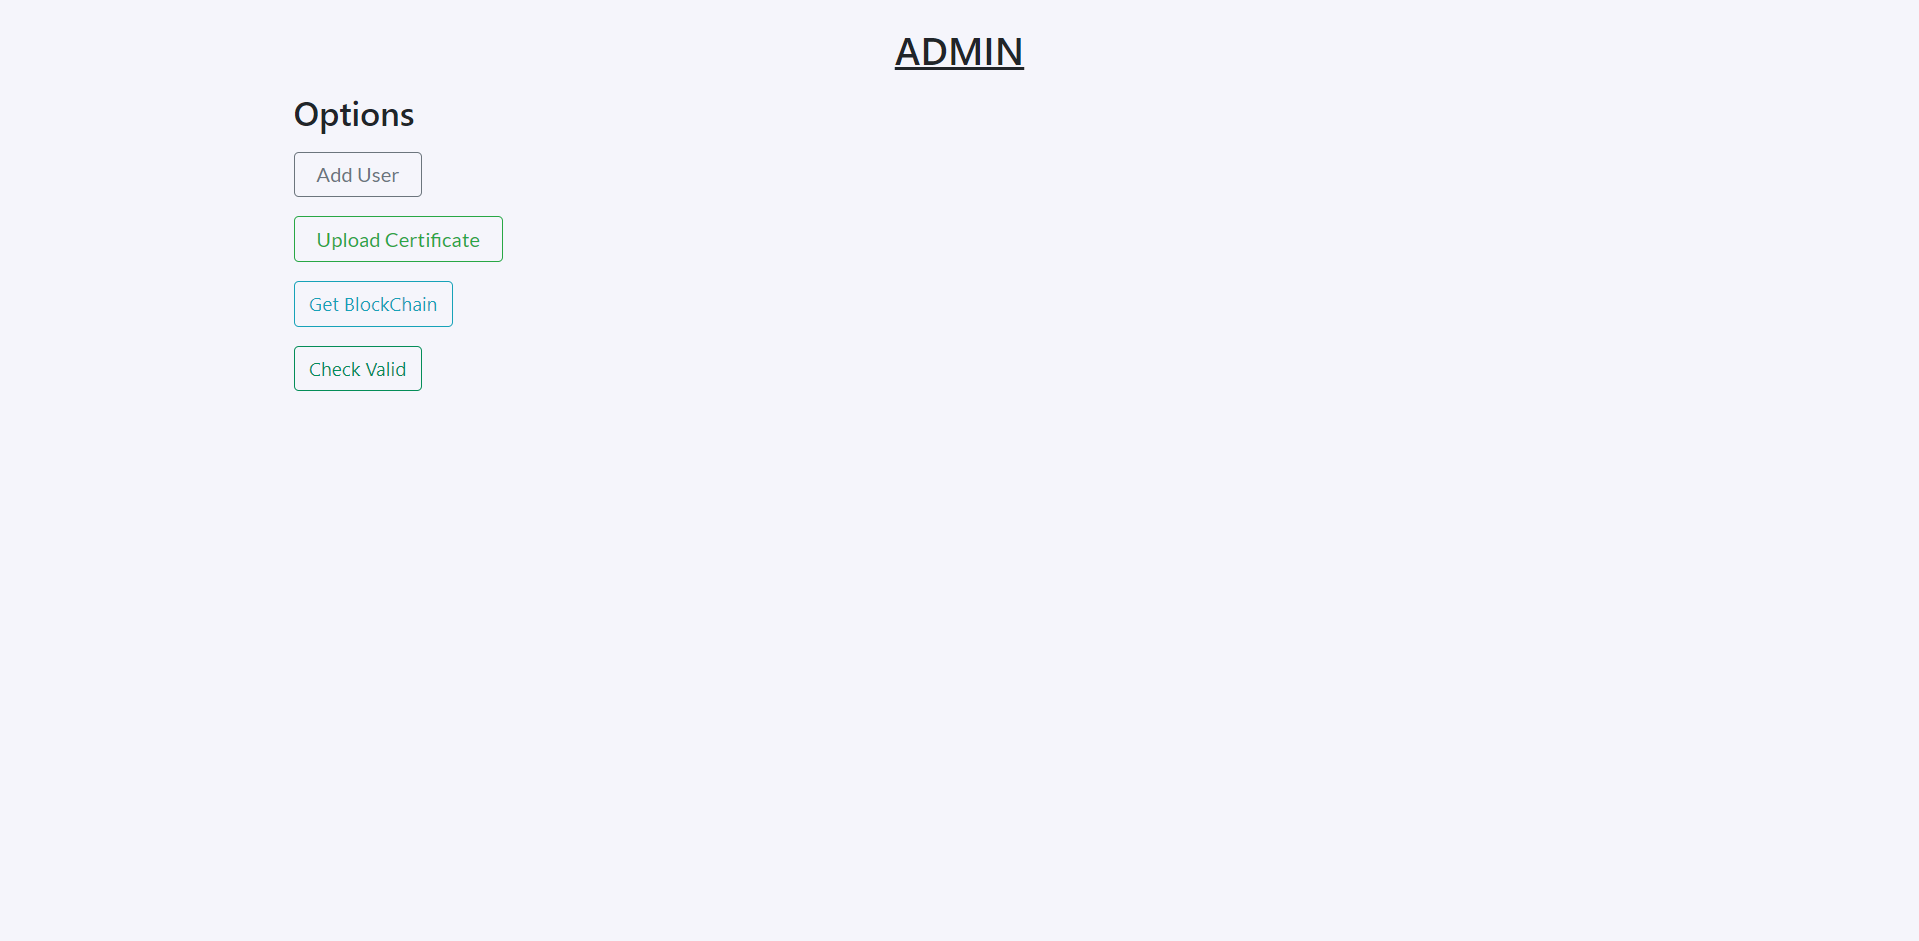
\includegraphics[scale=0.32]{images/Admin Page.png}\\[0.5cm]
    \caption{Admin Page Design}
    \label{fig:Admin Page}
\end{figure}

Admin Page is designed for admins to select the option between Get chain, Is chain valid, upload certificates, and add user.

\begin{figure}[H]
    \centering
    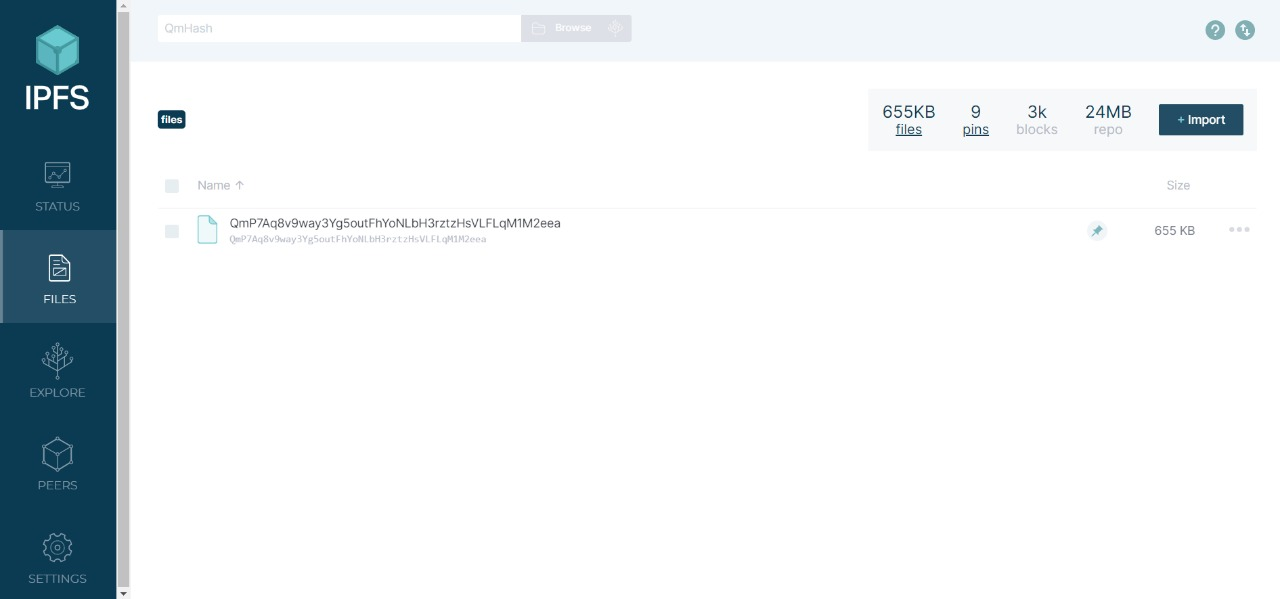
\includegraphics[scale=0.37]{images/ipfs-UI.jpeg}\\[0.5cm]
    \caption{IPFS Design}
    \label{fig:my_label}
\end{figure}

\subsection{Decentralized Storage Design}
\begin{enumerate}
    \item John wants to Upload file on IPFS.
    \item He encrypted it with Jinny's public key.
    \item He uploaded it onto the IPFS.
    \item File is available on the IPFS network.
    \item Jinny can access that file with her private key.
    \item No one else can decrypt the file.
\end{enumerate}

\begin{figure}[H]
    \centering
    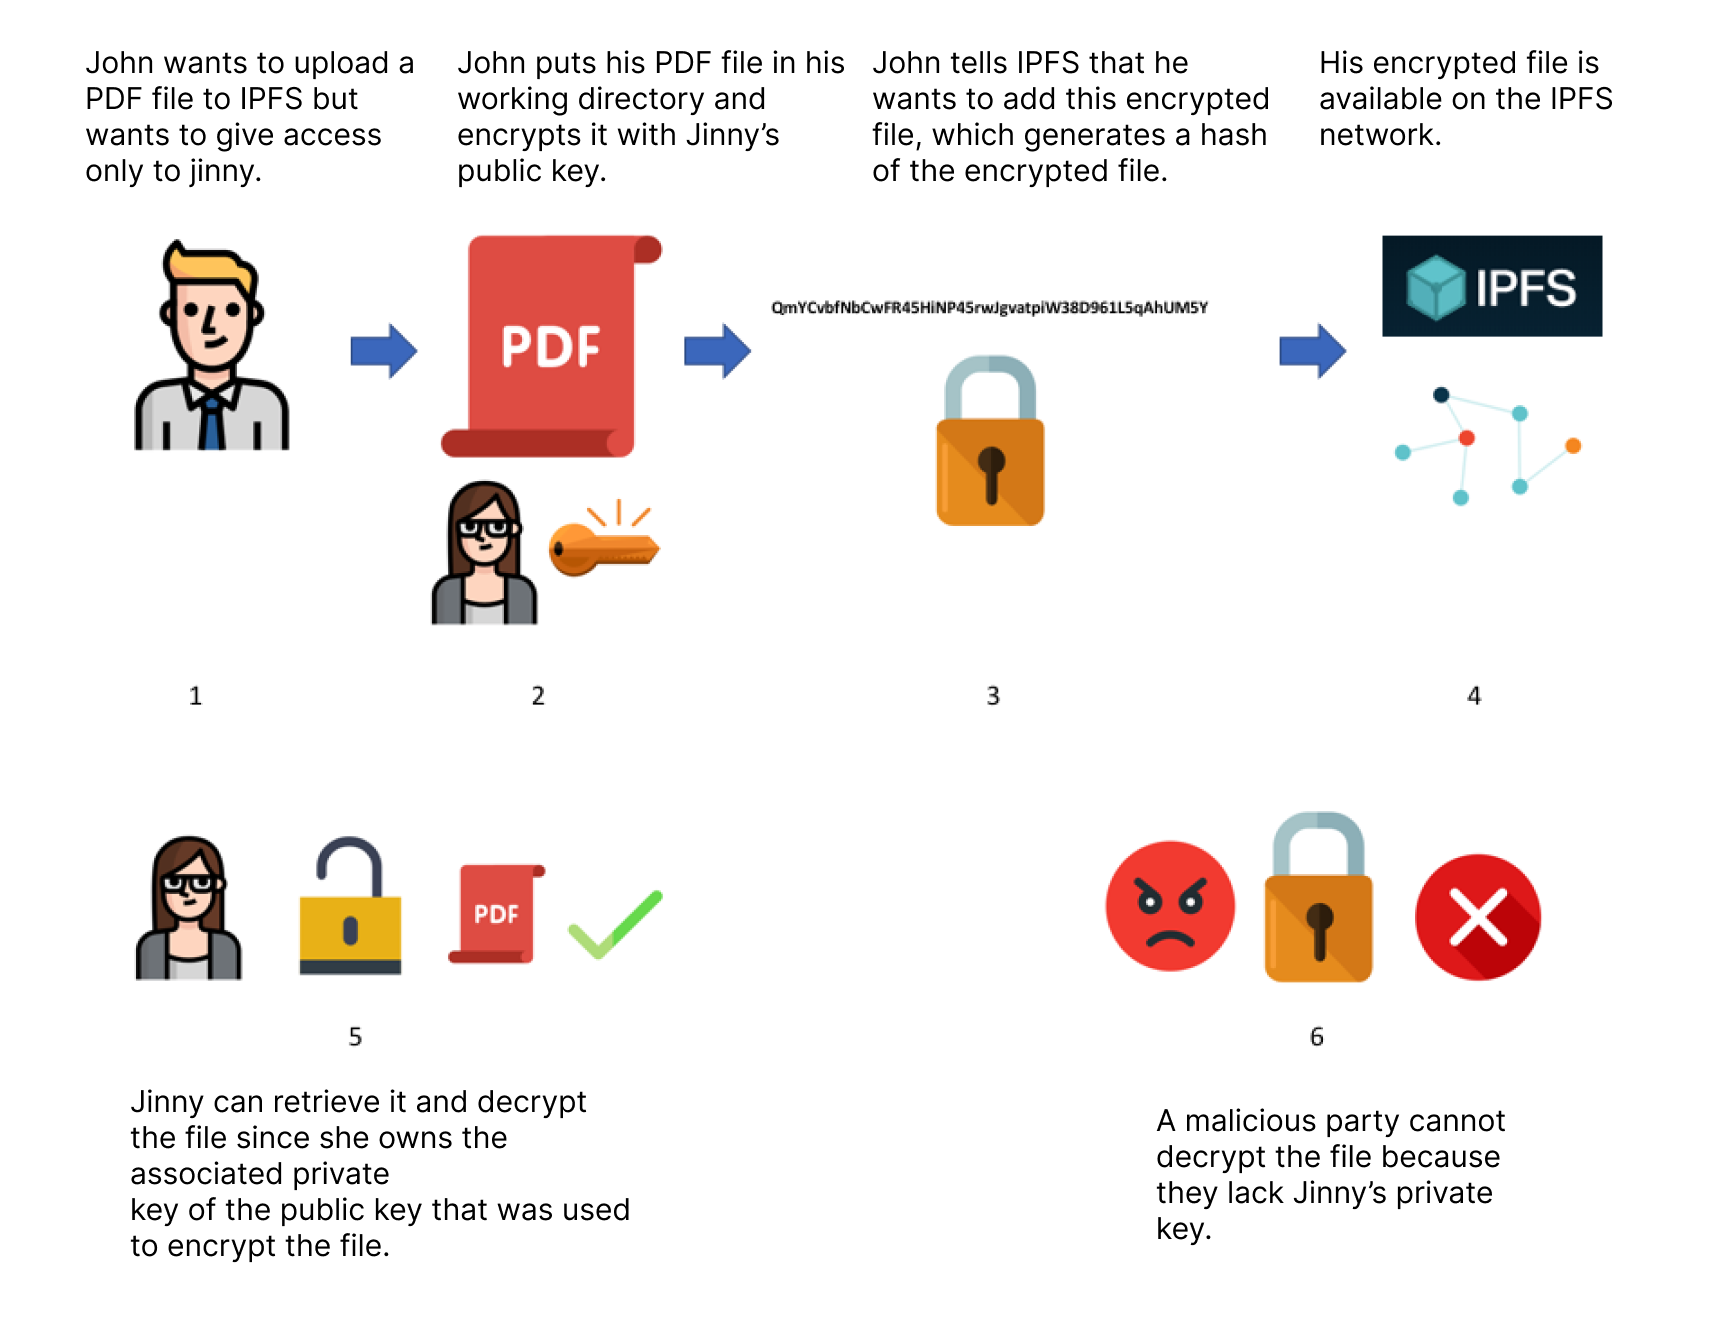
\includegraphics[scale=0.26]{images/ipfs_workflow.png}\\[0.5cm]
    \caption{IPFS Workflow}
    \label{fig:my_label}
\end{figure}

\subsection{Database Design}
% \subsubsection{ER Diagrams}
% \subsubsection{Normalization}
% \subsubsection{Database Connection Controls and Strings}
\begin{itemize}
    \item Student Table of handling database of students with their certificates:
    \begin{figure}[h]
        \centering
        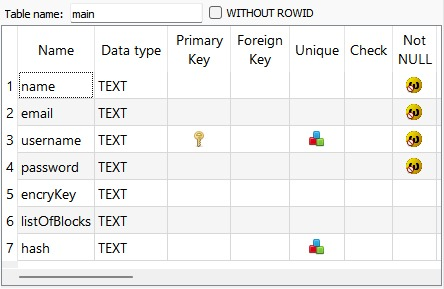
\includegraphics[scale=0.70]{images/Database Description.jpeg}\\[0.5cm]
        \caption{Student Database}
        \label{fig:Student Database}
    \end{figure}
    
    \item Table of saving blockchain in the database:
    \begin{figure}[h]
        \centering
        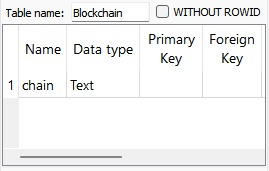
\includegraphics[scale=0.70]{images/2nd database description.jpeg}\\[0.5cm]
        \caption{Blockchain Table}
        \label{fig:Blockchain Table}
    \end{figure}

\end{itemize}




\subsection{Methodology}

We have chosen the \textbf{Waterfall model} as our \textbf{Systems Development Life Cycle} (SDLC) as it has been observed to best fit the nature of the research since it provides an easy to understand sequential and systematic process of developing the software that had the possibility of the changing requirements.

The waterfall model software development life cycle traditionally have the following five stages:
\begin{itemize}
    % \item \textbf{Planning:} Based on the analysis of the existing transcript management, it showed problems like: Record misplacement, Going back to multiple sources for validating data, High time consumption, Non-cost effective system, etc are there.
    % Hence, to overcome this, new transcript management system using Blockchain achieved the following:
    % Permanent Records, time efficiency, Secure data, Decentralized data, Easily traceable.
    % \item \textbf{Analysis:} To meet the users expectation, this application considered and adopted the college or university authorities as the end users since they are usually involved with the features and functionality of storing the students transcript.
    % \item \textbf{Design:} Designing a Transcript Management System as a software product is one of the most creative, innovative, complex processes and requires critical iterative thinking, understanding, and implementation of the design.
    % \item \textbf{Implementation:} As the phases are executed sequentially, all the components(Splash Page, Login Page, Select Faculty, Students details page, etc.) will be implemented on individual basis, and later will be integrated at different stages/levels. 
    % \item \textbf{Maintenance:} This software will be easy to maintain as, using blockchain for transcript Management, data will be decentralized and will be cost efficient. 
    \item \textbf{Data Collection of Transcripts:} To collect the transcript data to be stored in blocks and to observe the data through repeated careful listening.
    \item \textbf{Creation of Nodes:} Blocks of data are stored on nodes. To connect all the nodes on blockchain so they can constantly exchange the latest blockchain data with each other so that all nodes stay up to date.
    \item \textbf{Creation of Blocks:} To create blocks in the blockchain and identifying then with SHA256 values that will include encrypted transaction information from previous blocks and new transaction information.
    \item \textbf{Blockchain:} To build chain of blocks so that when a new transaction occurs, a block is added in the blockchain.
\end{itemize}

\begin{figure}[h]
    \centering
    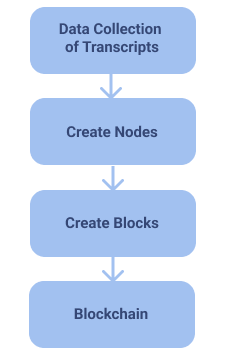
\includegraphics[scale=0.7]{images/Methodology.png}\\[0.5cm]
    \caption{Methodology of work}
    \label{fig:my_label}
\end{figure}

